%versi 2 (8-10-2016)
\chapter{Tinjauan Umum Perusahaan}
\label{chap:tinjauanperusahaan}
Bab ini akan membahas profil dan struktur perusahaan. Bab ini akan menjelaskan gambaran umum dari PT DNArtworks. Profil perusahaan akan menjelaskan sedikit sejarah perusahaan dan garis besar struktur dalamnya. Struktur perusahaan akan memberikan gambaran lebih jelas dari perusahaan dan tempat penulis mengerjakan proyek ini.

\section{Profil Perusahaan}
\label{sec:profilperusahaan} 
 PT DNArtworks Komunikasi Visual (DNArtworks, \href{https://dnartworks.co.id}{https://dnartworks.co.id}) adalah perusahaan grup konsultan yang menspesialisaikan dirinya pada pembangunan desain, \textit{brand}, situs web, maupun aplikasi \textit{mobile}. DNArtworks telah mengerjakan proyek dari berbagai klien, mulai dari individu, koperasi, hingga perusahaan-perusahaan ternama seperti Piaggio Indonesia, Fruit Tea Sosro, 5àsec, dan BP Indonesia.
 
 DNArtworks didirikan oleh Daniel Rahadian Nugroho pada bulan April 2013, di Brisbane, Australia, dan mengerjakan hanya jasa desain grafis. DNArtworks dibawa ke Indonesia di tahun 2015 dan sejak saat itu berkembang menjadi seperti saat ini. Dalam perjalanannya, muncul tim baru di dalam DNArtworks, yaitu Piktora. Piktora berfokus mengerjakan desain visual dari DNArtworks, sedangkan DNArtworks sendiri berfokus pada pembuatan situs web, aplikasi mobile, dan videografi. Satu rintisan terbaru dari DNArtworks adalah dipapier, yang berfokus pada jasa pembuatan undangan pernikahan, baik cetak maupun daring.

Secara internal, tim development dari DNArtworks dikenal dengan nama DNA Digital. Tim ini awalnya hanya diisi oleh satu orang alumni Teknik Informatika UNPAR, Sudarsono Sihotang. Dalam perjalanannya, Sudarsono memutuskan untuk pindah ke perusahaan lain, dan terjadi kekosongan pada DNA Digital. Sebagai gantinya, DNA Digital diisi oleh Pascal Alfadian Nugroho, dibantu beberapa mahasiswa magang dan alumni.

\section{Struktur Perusahaan}
\label{sec:strukturperusahaan}

Karena jumlah personel tim cukup banyak, maka bagan struktur organisasi dibagi dua, yaitu DNArtworks dan DNA Digital.

\begin{sidewaysfigure}[ht]
\center
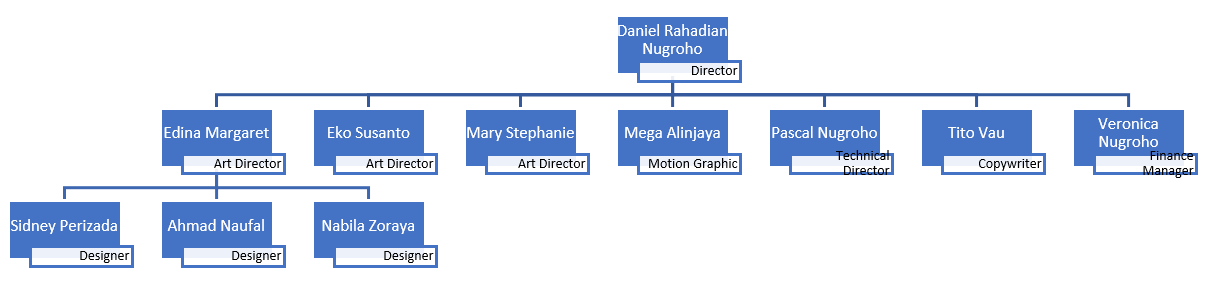
\includegraphics[width=\textwidth,height=\textheight,keepaspectratio]{Gambar/Struktur DNArtworks.PNG}
\caption{Struktur DNArtworks.}
    \label{img:strukturdnartworks}
\end{sidewaysfigure}

DNArtworks memiliki struktur seperti di Gambar \ref{img:strukturdnartworks}. Ketua DNArtworks bertanggung jawab langsung ke beberapa kepala bagian di perusahaan. Kepala bagian sendiri memiliki bidangnya masing-masing dan saling berhubungan satu sama lain. Salah satu contohnya adalah koordinasi dari Edina Margaret yang membantu Tim Teknis dalam desain UI (\textit{User Interface}) dalam beberapa proyek. Selain tim teknis, mayoritas personel ada di kantor utama yang berada di Jakarta.

\begin{figure}[H]
\center
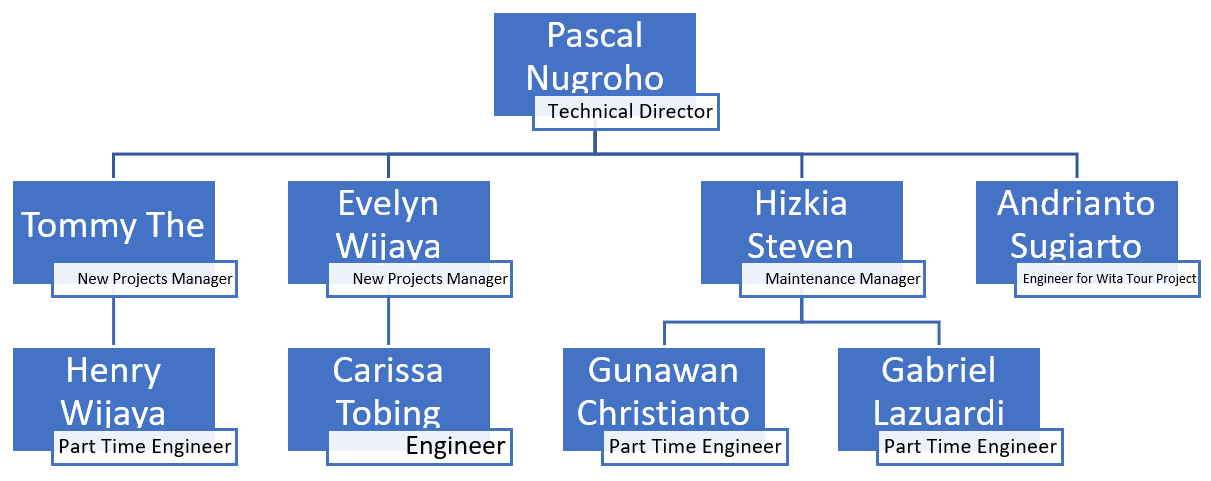
\includegraphics[width=\textwidth,height=\textheight,keepaspectratio]{Gambar/Struktur DNA Digital.PNG}
\caption{Struktur DNA Digital.}
\label{img:strukturdnadigital}
\end{figure}

DNArtworks memiliki tim teknis di bawah Pascal Nugroho dengan struktur seperti di Gambar \ref{img:strukturdnadigital}. Tim ini yang bertanggung jawab dalam pembangunan proyek seperti \textit{website} dan aplikasi \textit{mobile}. Struktur DNA Digital sering kali berubah-ubah karena menyesuaikan dengan proyek yang ditangani. Oleh karena itu, struktur yang ada di atas hanya gambaran besar karena pada dasarnya, posisi Pascal dan 4 orang yang berada di bawah beliau langsung tidak berubah-ubah.

